\documentclass[tikz,border=12pt]{standalone}
\usetikzlibrary{arrows.meta,positioning}
\definecolor{pink}{HTML}{F72585}\definecolor{green}{HTML}{51CF66}\definecolor{gray}{HTML}{ADB5BD}\definecolor{ink}{HTML}{E9ECEF}\definecolor{panel}{HTML}{211C1D}
\begin{document}
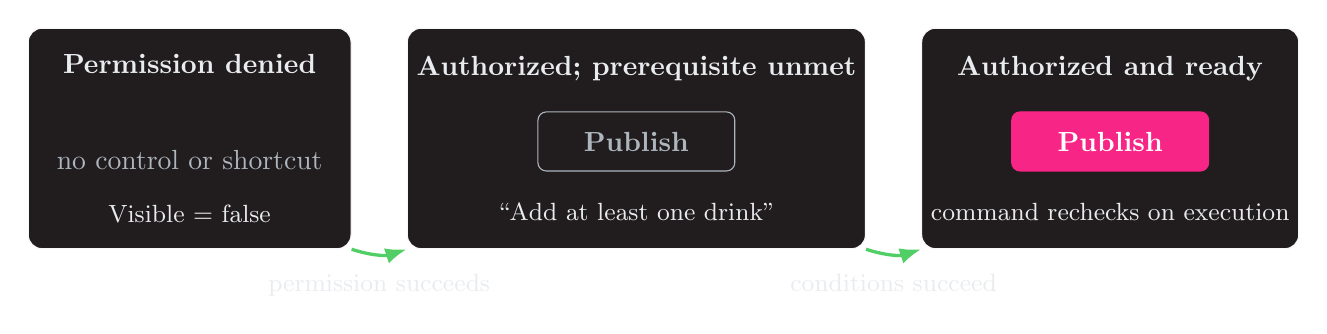
\begin{tikzpicture}[text=ink,panel/.style={rounded corners=5pt,draw=ink!35,fill=panel,minimum width=4.1cm,minimum height=2.8cm,align=center},button/.style={rounded corners=3pt,minimum width=2.5cm,minimum height=.75cm,font=\bfseries}]
 \node[panel] (hidden) at (0,0) {\textbf{Permission denied}\\[.8cm]\textcolor{gray}{no control or shortcut}\\[.25cm]\small Visible = false};
 \node[panel,right=.7cm of hidden] (disabled) {\textbf{Authorized; prerequisite unmet}\\[.35cm]\tikz\node[button,draw=gray,fill=panel,text=gray]{Publish};\\[.2cm]\small ``Add at least one drink''};
 \node[panel,right=.7cm of disabled] (enabled) {\textbf{Authorized and ready}\\[.35cm]\tikz\node[button,draw=pink,fill=pink,text=white]{Publish};\\[.2cm]\small command rechecks on execution};
 \draw[-{Latex[length=2.7mm]},very thick,green] (hidden.south east) to[bend right=18] node[below=.12cm,font=\small,text=ink]{permission succeeds} (disabled.south west);
 \draw[-{Latex[length=2.7mm]},very thick,green] (disabled.south east) to[bend right=18] node[below=.12cm,font=\small,text=ink]{conditions succeed} (enabled.south west);
\end{tikzpicture}
\end{document}
